\DocumentMetadata{tagging=on}
\documentclass{article}

\usepackage{listings}
\usepackage{tikz}
\usetikzlibrary{tikzmark}
\usetikzmarklibrary{listings}

\title{tikzmark tagging test -- listings library}

\begin{document}

\tikzset{tikzmark prefix=ex6-}
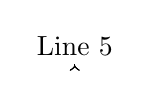
\begin{tikzpicture}[remember picture]
\foreach \k in {0,...,7} {
\iftikzmark{line-code-\k-start}{\fill[red,overlay] (pic
cs:line-code-\k-start) circle[radius=4pt];}{\message{No start
for \k}}
\iftikzmark{line-code-\k-end}{\fill[blue,overlay] (pic
cs:line-code-\k-end) circle[radius=2pt];}{\message{No end for
\k}}
\iftikzmark{line-code-\k-first}{\fill[green,overlay] (pic
cs:line-code-\k-first) circle[radius=2pt];}{\message{No first
for \k}}
}
\draw[->,overlay] (0,0) -- (pic cs:line-code-5-first);
\draw[->,overlay] (0,0) -- (pic cs:line-code-5-start);
\draw[->,overlay] (0,0) -- (pic cs:line-code-5-end);
\node[above] at (0,0) {Line 5};
\end{tikzpicture}
\begin{lstlisting}[language=c,name=code,numbers=left]
#include <stdio.h>
int main(void)
{
printf("hello, world\n");
return 0;
}
\end{lstlisting}

\end{document}